\chapter{System Evaluation}\label{chap:eval}
One of the aims stated for this study as listed in the Chapter~\ref{sec:Introduction} was to write a Python application with scalability in mind. Therefore this chapter is devoted to present a 1000 feet view of the application so that the implementation described in prior chapters could be taken as only one of possibilities to realize the intended system characteristics and functionality.   

\section{Final result presentation}\label{sec:result} 
The web interface of SmartNotes is a simple internationalized application that read about the project and access iterated users to the functionality. Currently it includes only creating a SmatNotes account by using the Google Account as described in Section~\ref{subsec:ismartnotes_activation} and receiving an activation key. That process is straight forward and it is presented in Figures A, B, and C. Finally the user can pass the activation code to  the iSmartNotes
application to take the advantage of synchronization feature. It allows to the users as described in Section~\ref{sec:functionality_descr} to fork on their notes and perform a synchronization when the network connection is available.
The main iSmartNotes window is presented in Figure~\ref{fig:ismartnotes_window}. It has a simple text area where the notes can be edited and sync button that dependently on the network connectivity will perform synchronization on local machine or additiionly using the SmartNotes interface illustrated in Figure~\ref{fig:smartnotes_components}. 
\begin{figure}[ht]
  \begin{center}
    \subfigure[\textbf{Without mailing service}.]{\label{fig:sm_main}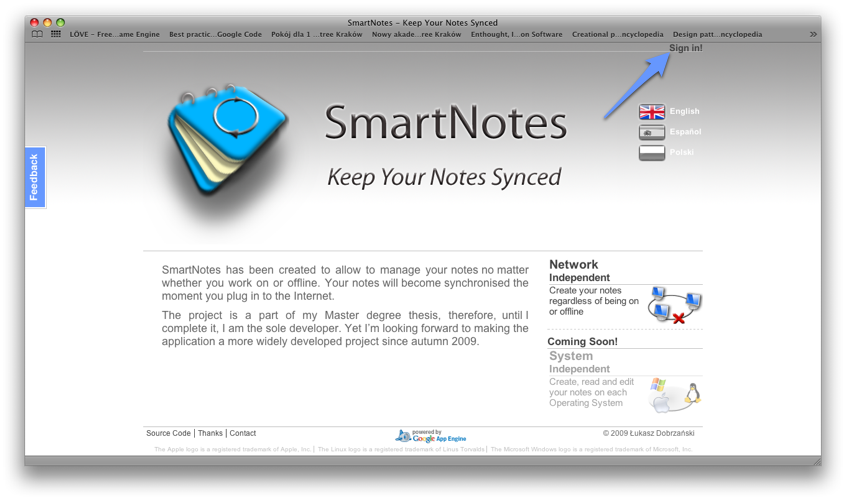
\includegraphics[scale=0.5]{img/SNmain_page.png}}
    \subfigure[\textbf{With mailing service}.]{\label{fig:sm_signin}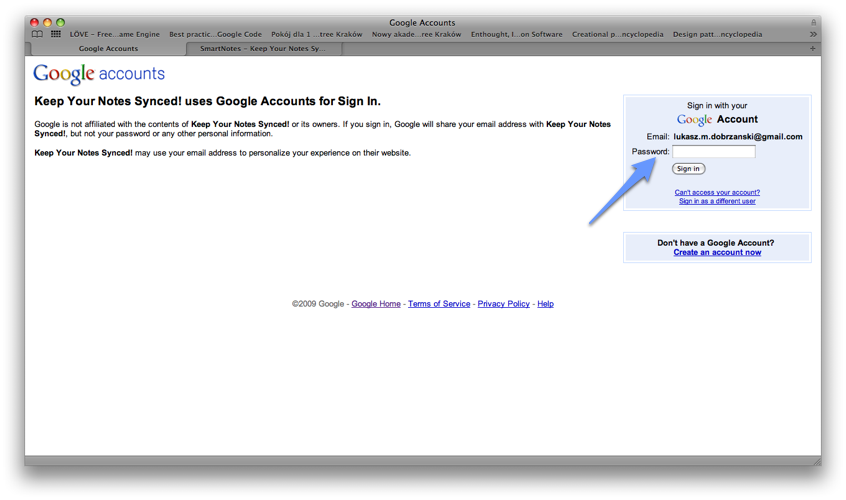
\includegraphics[scale=0.24]{img/SN_signin.png}}
    \subfigure[\textbf{With mailing service}.]{\label{fig:sm_getSNkey}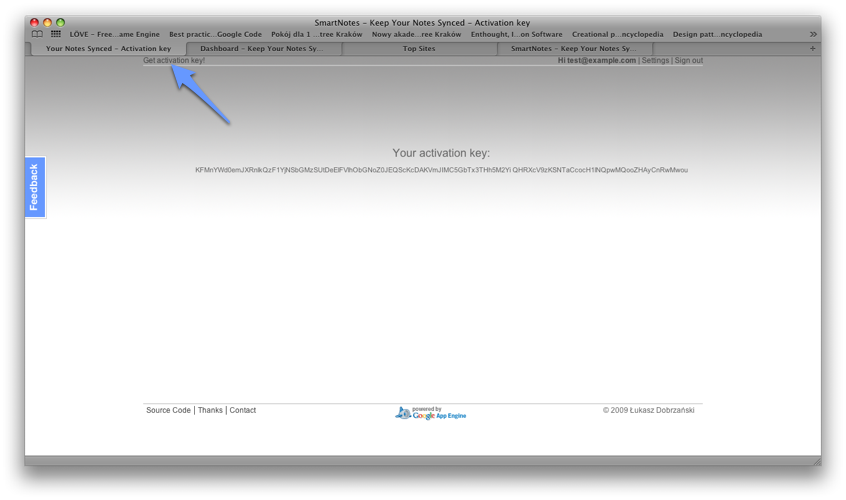
\includegraphics[scale=0.24]{img/SNget_activation_key.png}}
  \end{center}
  \caption{Simulated monthly cost division of resources expected to be used by one million of SmartNotes users on Google App Engine.}
  \label{fig:sn_web_interface}
\end{figure}


        
\begin{figure}[ht]
\begin{center}
\includegraphics[scale=0.5]{img/SN_ismartnotes_window.pdf}
\caption{The view on the iSmartNotes application window.}
\label{fig:ismartnotes_window}
\end{center}
\end{figure}

\section{Performance tests}\label{sec:performance} 